$passoptions.latex()$
\documentclass{article}

\usepackage[nonatbib, final]{nips_2017}

\usepackage[utf8]{inputenc}
\usepackage[T1]{fontenc}
\usepackage{hyperref}
\usepackage{url}
\usepackage{booktabs}
\usepackage{amsfonts}
\usepackage{amsmath}
\usepackage{nicefrac}
\usepackage{microtype}
\usepackage{subfiles}
\usepackage{xcolor}
\usepackage{multirow}
\usepackage{enumerate}
\usepackage{subfiles}
\usepackage{multirow}
\usepackage{graphicx}
\usepackage{subfiles}

$font-settings.latex()$
$common.latex()$
$hypersetup.latex()$

\newcommand\todo[1]{\textcolor{red}{[[#1]]}}
\newcommand\mc[1]{\mathcal{#1}}
\newcommand*\samethanks[1][\value{footnote}]{\footnotemark[#1]}

\newcommand{\kq}{q}
\newcommand{\km}{k}
\newcommand{\vq}{o}
\newcommand{\vm}{m}
\newcommand{\Wkq}{W_q}
\newcommand{\Wkm}{W_k}
\newcommand{\Wvq}{W_o}
\newcommand{\Wvm}{W_m}
\newcommand{\dmodel}{d_{\text{model}}}
\newcommand{\dffn}{d_{\text{ffn}}}
\newcommand{\dff}{d_{\text{ff}}}
\newcommand{\mbf}[1]{\mathbf{#1}}
\newcommand\concat[3]{\left[#1 \parallel_#3 #2\right]}

\title{Attention Is All You Need}
\author{
  \AND
  Ashish Vaswani\thanks{Equal contribution. Listing order is random. Jakob proposed replacing RNNs with self-attention and started the effort to evaluate this idea.
Ashish, with Illia, designed and implemented the first Transformer models and has been crucially involved in every aspect of this work. Noam proposed scaled dot-product attention, multi-head attention and the parameter-free position representation and became the other person involved in nearly every detail. Niki designed, implemented, tuned and evaluated countless model variants in our original codebase and tensor2tensor. Llion also experimented with novel model variants, was responsible for our initial codebase, and efficient inference and visualizations. Lukasz and Aidan spent countless long days designing various parts of and implementing tensor2tensor, replacing our earlier codebase, greatly improving results and massively accelerating our research.
}\\
  Google Brain\\
  \texttt{avaswani@google.com}\\
  \And
  Noam Shazeer\footnotemark[1]\\
  Google Brain\\
  \texttt{noam@google.com}\\
  \And
  Niki Parmar\footnotemark[1]\\
  Google Research\\
  \texttt{nikip@google.com}\\  
  \And
  Jakob Uszkoreit\footnotemark[1]\\
  Google Research\\
  \texttt{usz@google.com}\\
  \And  
  Llion Jones\footnotemark[1]\\
  Google Research\\
  \texttt{llion@google.com}\\   
  \And
  Aidan N. Gomez\footnotemark[1] \hspace{1.7mm}\thanks{Work performed while at Google Brain.}\\
  University of Toronto\\
  \texttt{aidan@cs.toronto.edu}
  \And
  {\L}ukasz Kaiser\footnotemark[1]\\
  Google Brain\\
  \texttt{lukaszkaiser@google.com}\\
  \And
  Illia Polosukhin\footnotemark[1]\hspace{1.7mm} \thanks{Work performed while at Google Research.}\\
  \texttt{illia.polosukhin@gmail.com}\\  
}

\begin{document}

\maketitle

\begin{abstract}
The dominant sequence transduction models are based on complex recurrent or convolutional neural networks that include an encoder and a decoder. The best performing models also connect the encoder and decoder through an attention mechanism. We propose a new simple network architecture, the Transformer, based solely on attention mechanisms, dispensing with recurrence and convolutions entirely. Experiments on two machine translation tasks show these models to be superior in quality while being  more parallelizable and requiring significantly less time to train. Our model achieves 28.4 BLEU on the WMT 2014 English-to-German translation task, improving over the existing best results, including ensembles, by over 2 BLEU.  On the WMT 2014 English-to-French translation task, our model establishes a new single-model state-of-the-art BLEU score of 41.8 after training for 3.5 days on eight GPUs, a small fraction of the training costs of the best models from the literature. We show that the Transformer generalizes well to other tasks by applying it successfully to English constituency parsing  both with large and limited training data.
\end{abstract}

$body$

\pagebreak
\section*{Attention Visualizations}\label{sec:viz-att}
\begin{figure*}[h]
{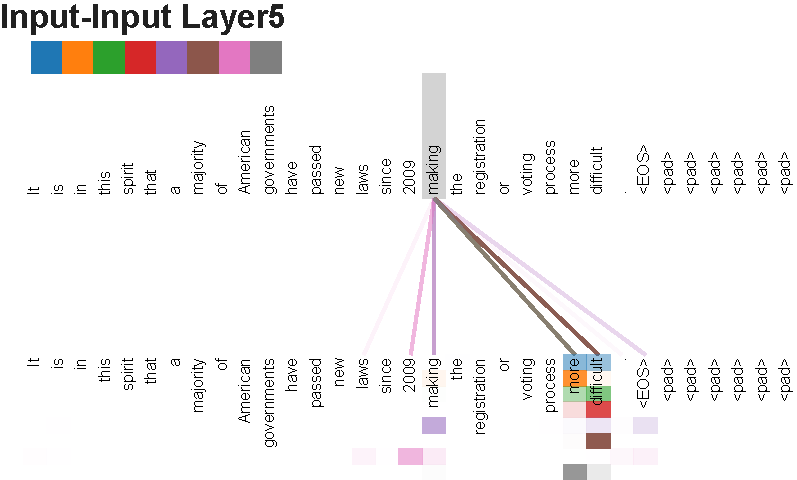
\includegraphics[width=\textwidth, trim=0 0 0 36, clip]{./vis/making_more_difficult5_new.pdf}}
\caption{An example of the attention mechanism following long-distance dependencies in the encoder self-attention in layer 5 of 6. Many of the attention heads attend to a distant dependency of the verb `making', completing the phrase `making...more difficult'.  Attentions here shown only for the word `making'. Different colors represent different heads. Best viewed in color.}
\end{figure*}

\begin{figure*}
{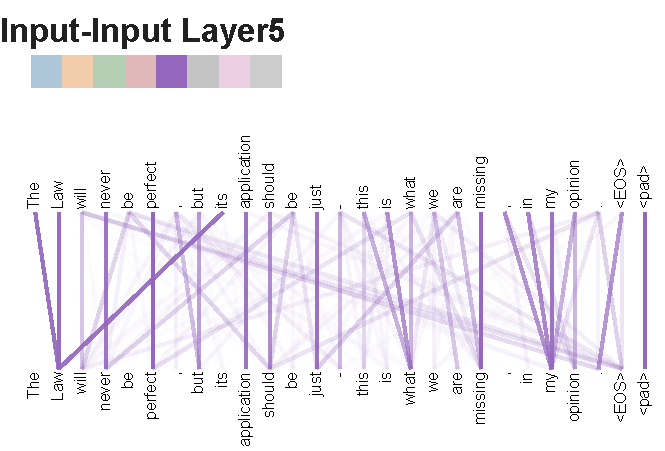
\includegraphics[width=\textwidth, trim=0 0 0 45, clip]{./vis/anaphora_resolution_new.pdf}}
{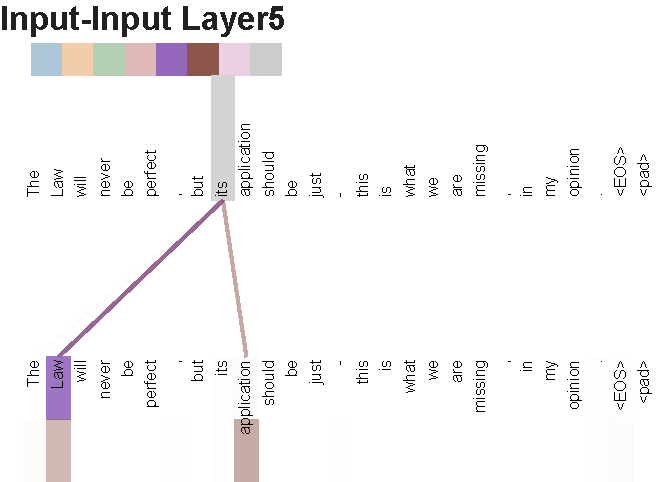
\includegraphics[width=\textwidth, trim=0 0 0 37, clip]{./vis/anaphora_resolution2_new.pdf}}
\caption{Two attention heads, also in layer 5 of 6, apparently involved in anaphora resolution. Top: Full attentions for head 5. Bottom: Isolated attentions from just the word `its' for attention heads 5 and 6. Note that the attentions are very sharp for this word.}
\end{figure*}

\begin{figure*}
{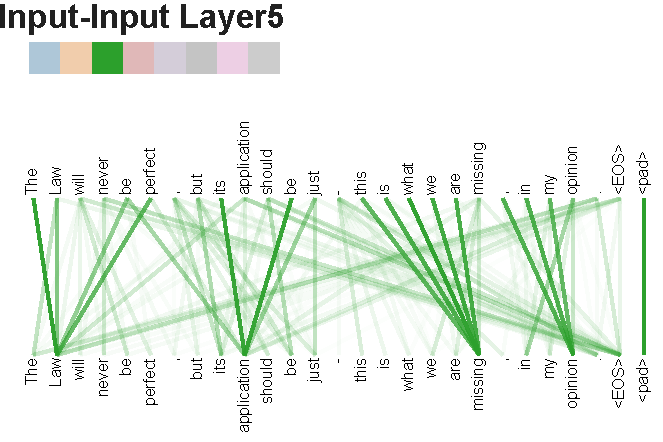
\includegraphics[width=\textwidth, trim=0 0 0 36, clip]{./vis/attending_to_head_new.pdf}}
{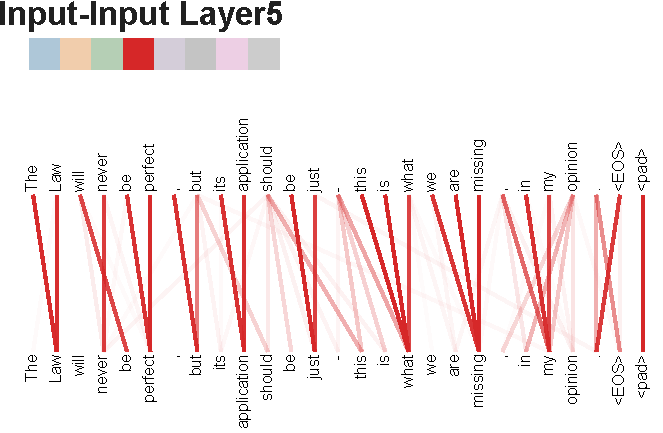
\includegraphics[width=\textwidth, trim=0 0 0 36, clip]{./vis/attending_to_head2_new.pdf}}
\caption{Many of the attention heads exhibit behaviour that seems related to the structure of the sentence. We give two such examples above, from two different heads from the encoder self-attention at layer 5 of 6. The heads clearly learned to perform different tasks.}
\end{figure*}


\end{document}